% Appendix D -- the skill span.
\section{The span battery, in full}
\label{app:battery}

\S\ref{sec:onepos} is a negative result about a probe, not about a model. The
probe fails because one position cannot hold a decision that occupies hundreds
of tokens. The obvious repair is to stop using one position, and the natural
place to use instead is the one group of positions whose size grows with the
document: the document's own tokens.

\paragraph{The receiver.} The donor is the with-document forward; the receiver
is the \emph{same prompt} with the document's tokens overwritten, one for one,
by the tokens of \emph{one fixed clinical skill document}---the same document
for every instance and every skill, and the gold document of none of them.

Both halves of that choice were forced by measurement. It has to be fixed,
because a receiver built from each skill's own paired control makes the
receiver's states depend on the instance, and then every arm of the form
$h_{\text{recv}} + (\cdot)$ inherits an instance-dependent floor; measured, the
with-document states vary across a skill's instances by a relative
$3.5\times10^{-3}$ while such a receiver's vary by $0.36$. We use a
\emph{clinical} document rather than neutral prose because it is the same
condition the behavioural runs call
``wrong skill'', so the receiver's baseline means what the paper's presence
effect means; \S\ref{sec:plausible} measures the two side by side and finds them
close ($0.150$ against $0.250$, $n=40$, overlapping intervals).

Length-matching is not a refinement here either, it is the whole experiment. An
earlier version of this run used the no-document
prompt, which is some $900$ tokens shorter, and aligned the spans by their ends;
the real arm and the wrong-document arm then both read $0.200$---the signature
of two arms broken in the same way by a rotary phase shift, which is easy to
read as an absent effect. With a matched receiver every position keeps its
index, the two sequences are identical outside the span, and the question span
is verified token-identical between donor and receiver before anything is
patched.

Because the receiver already holds a document, the substitution obeys
$h_{\text{recv}}(\text{span}) + \dvec(\text{span}) = h_{\text{skill}}(\text{span})$: it is $h_{\text{recv}} + \dvec$ at $\alpha=1$. That is
what makes the rest of this section possible.

\paragraph{It carries, completely.} Figure~\ref{fig:channels} puts the two
channels side by side on the same model and the same decomposition. At the last
prompt position, five arms---including replacing the entire state with the
with-document one---sit between $0.050$ and $0.150$ against a no-document
baseline of $0.050$. Over the document's own span, after the instrument fix,
the corresponding span content matrix gives $1.00$ against a receiver at $0.00$ ($n=16$, four
calculators).

Before the fix the same panel read $0.950$ on twenty items, $\rho = 1.06$: the
transplant and the document disagreed on one item and the transplant got it
right. The honest reading of every $\rho$ near or above $1$ here is
``indistinguishable from having the document in the prompt''.



\paragraph{How deep the handover works (before the fix).} Transplanting the \emph{document's own}
states over the same construction recovers the document's entire effect through
layer 12 and then falls off a cliff (Table~\ref{tab:realspandepth}). Layer 0 is
close to tautological---a layer's output over the document's tokens is not far
from putting those tokens back---so the load-bearing entries are layers 8 and
12, a third of the way into
the network, where the receiver has already processed eight or twelve blocks'
worth of filler in those positions and the transplant still recovers
everything. Past layer 14 a single layer's worth stops being enough: $\rho =
0.14$ at 15 and 16, and $0.00$ at 24 and 30. Writing
the span at \emph{every} layer at once returns it to $\rho = 1.00$, so what
fails past layer 14 is the handover at one depth, not the mechanism.

\paragraph{The profile replicates; its one anomaly does not.} We ran the sweep a
second time on the same items against the other receiver---the single fixed
wrong skill rather than each skill's paired control---and the two agree wherever
the first is well behaved: $+1.00$ against $+1.00$ at layer 0, $+1.06$ against
$+1.07$ at 4, $+1.03$ against $+1.14$ at 8, $+0.81$ against $+1.00$ at 12
(Table~\ref{tab:realspanfixed}). The single bump in the first run, $\rho=0.07$
at layer 18 against $0.29$ at 20, does not survive: the replication gives $+0.16$
at layer 20, below its own layer 16. We read the profile and not the individual
layers, and we read that bump as noise.



The surviving window is a window in \emph{relative} depth: layers 0--12 of 36
here, 0--10 of 28 on the synthetic tier, both about a third of the way in.



\paragraph{It behaves like a mechanism, not like a perturbation.} Four
controls, all at layer $8$, all in Figure~\ref{fig:channels}, and all read on
the calculators a wrong document never rescues.

\emph{Dose}: after the fix, $\alpha = 0.4, 0.5, 0.55, 0.6, 0.7, 1, 2$ give
$\rho = 0.06, 0.00, 0.06, 0.62, 0.94, 1.00, 0.81$ ($n=16$). The transition is a
step and not a ramp---half the content is no better than none of it, since the
state is then a midpoint between two coherent documents and corresponds to
neither---and overshooting costs a little. An injection that merely had to be
large would show neither. Before the fix the same sweep read $0.17, 0.03, 0.17,
0.88, 0.97, 1.00$ ($n=30$), and a coarser one $0.06, 1.06, 1.06, 0.89$ at
$\alpha = 0.5, 0.75, 1, 2$ with the per-position rescaled doses coinciding
($0.06$ and $0.89$ both ways).

\emph{Transfer}: after the fix, another skill's vector over the prefix the two
documents share gives $0.19$ against $0.94$ for this skill's own vector on the
same positions ($n=16$), and on forty calculators a donor from another family
$0.06$ and one from the same family $0.06$ against $0.73$. Before the fix, the
mean content vector of a \emph{different} skill, written over the prefix the two
documents share, gave $\rho = 0.06$ against $1.00$ for
this document's own vector written over \emph{the same positions}. Because every
skill's vector is taken against the same fixed control, this arm is exactly that
skill's own span states rather than a hybrid, so it is the cleanest form the
transfer test can take; and the paired control is what makes it a statement about
content rather than about how many positions were patched.

\emph{Order}: the same vectors, permuted across the span's own positions, give
$\rho = 0.00$ ($n=16$) and $0.08$ on forty calculators after the fix ($0.12$
before). The span is not a bag---which position holds which part of the
document is most of the effect.

\emph{Norm}: Gaussian noise rescaled to each position's $\|\dvec\|$ gives
$\rho = 0.00$, exactly the receiver ($0.10$ on forty calculators). The effect is not a consequence of writing
something large into those positions.

\paragraph{The split these four are read on, and why it is not cherry-picking.}
On four of the ten calculators the receiver---a wrong clinical document---already
solves the items. Before the fix every span arm worked there: a related-skill
donor scored $\rho = 0.71$, an unrelated one $0.43$ and norm-matched
\emph{noise} $0.14$, against $0.00$, $0.06$ and $0.00$ on the five where the
receiver scores zero, and pooling the two groups turned a null transfer arm into
an apparent $\rho = 0.38$. After the fix six calculators fall on that side;
noise no longer works there ($0.00$, $n=24$) but another skill's vector still
reads $0.47$ against $0.19$ on the four restricted calculators: there the wrong
document in the slot was leading the model astray, and a coherent replacement
lets it fall back on a formula it already knows.

The split conditions on the \emph{receiver}, which is a control, and on no
intervention arm, so it cannot manufacture the contrast it is used to report; and
it is taken per calculator rather than per instance because ``this model can do
this calculator unaided'' is a property of the calculator. Table~\ref{tab:battery-all}
gives every arm on all forty items for comparison.

\paragraph{It replicates on four times as many skills.} The ten calculators
above are the ten with the most rescued instances, and twenty items from five
calculators is the single most obvious reason to stop reading. We therefore ran
the battery on \emph{forty} calculators, recomputing the restriction inside the
larger set rather than carrying it over. Of the forty, fifteen are calculators
the wrong document never rescues, which leaves $60$ items---three times the
original---and every arm holds (Table~\ref{tab:big40}): the document's own
vector recovers $\rho = 0.87$, the same vector over only the prefix another skill's document shares $0.73$, half a dose
$0.06$, a donor from another family $0.06$, permutation of the span's own
positions $0.08$, and norm-matched noise $0.10$, against a null arm at exactly
$0.00$ and a receiver at exactly $0.000$, and a donor from the same family
$0.06$ (rerun after the instrument fix). The separation is
between $0.87$ and at most $0.10$, on three times the material, with
item-level intervals as identified in the main-text caption.



\paragraph{And it fails where the document fails (before the fix).} On the
persistent-failure cell---items the gold document does \emph{not} rescue---the
same transplant at the same layer gives $0.100$, equal to the receiver's $0.100$,
against the document's own $0.025$ ($n=40$, ten calculators; the null arm read
$0.150$ in this run). The channel transports what the document does, including doing
nothing. An arm that only ever helped would be consistent with a generic ``try
harder'' effect; this one is not.

\paragraph{Why it can carry when a single position cannot.} The span is $415$ to
$1{,}630$ positions wide on the forty calculators, the same order as the answer it has to support. This is the
positive half of \S\ref{sec:onepos}'s capacity statement, and the two together
give the rule the paper is built on: \emph{a patch transports what fits in the
positions it is given}. A one-token answer fits at one position; a chain of
thought fits nowhere except on a group of positions as large as the document
itself.


\begin{table}[tbp]
\caption{Behaviour on the real skills, Qwen3-8B, all three arms on the same
$1{,}100$ items, CIs bootstrapped over the 55 calculators. The presence effect
(wrong skill minus no skill) is a clean zero, so the $+39.7$pp is content.}
\label{tab:behaviour}
\centering
\small
\begin{tabular}{lrcc}
\toprule
& $n$ & accuracy & 95\% CI \\
\midrule
gold skill                & 1100 & 74.2\% & [65.8, 81.8] \\
no skill                  & 1100 & 34.5\% & [26.5, 42.8] \\
wrong skill (length-matched) & 1100 & 31.5\% & [23.7, 39.5] \\
\midrule
gold $-$ no skill         & 1100 & $+39.7$pp & [$+31.7$, $+47.7$] \\
gold $-$ wrong skill      & 1100 & $+42.6$pp & [$+34.7$, $+50.5$] \\
\textbf{presence: wrong $-$ no skill} & 1100 & $\mathbf{-2.9}$\textbf{pp} & [$-8.8$, $+3.0$] \\
\bottomrule
\end{tabular}
\end{table}

\begin{table*}[tbp]
\caption{The document-span transplant by layer. Qwen3-8B, 55 third-party
clinical skills, the $40$ rescued items, the full chain of thought decoded and
graded by the task's own scorer. The receiver is the with-skill prompt with the
document's tokens replaced by a filler document, before the instrument fix, so it is the same length and
every transplanted position keeps its rotary phase. Restricted, as everywhere in
this section, to the calculators the receiver never solves. This sweep used each
skill's paired control as the filler and the battery of \S\ref{sec:battery} the
single fixed one; over all forty items the three baselines agree to within
$0.01$ across the two ($0.175$/$0.025$/$0.950$ against $0.167$/$0.028$/$0.944$),
so the profile does not depend on that choice---the unrestricted version is
Table~\ref{tab:realspan-all}. The no-op arm---the receiver's own states written
back into the receiver---is reported wherever it was run and must equal the
receiver's baseline; it does, at every layer.}
\label{tab:realspandepth}
\centering
\small
\begin{tabular}{@{}rccc@{}}
\toprule
layer & accuracy & CI$_{95}$ & fraction of the document's own effect \\
\midrule
0 & $0.875$ & $[0.713,\,1.000]$ & $+1.00$ \quad\tiny(no-op arm 0.000) \\
4 & $0.938$ & $[0.819,\,1.000]$ & $+1.07$ \\
8 & $1.000$ & $[1.000,\,1.000]$ & $+1.14$ \\
12 & $0.875$ & $[0.713,\,1.000]$ & $+1.00$ \quad\tiny(no-op arm 0.000) \\
13 & $0.625$ & $[0.388,\,0.862]$ & $+0.71$ \quad\tiny(no-op arm 0.000) \\
14 & $0.688$ & $[0.460,\,0.915]$ & $+0.79$ \quad\tiny(no-op arm 0.000) \\
15 & $0.125$ & $[0.000,\,0.287]$ & $+0.14$ \quad\tiny(no-op arm 0.000) \\
16 & $0.125$ & $[0.000,\,0.287]$ & $+0.14$ \quad\tiny(no-op arm 0.000) \\
18 & $0.062$ & $[0.000,\,0.181]$ & $+0.07$ \quad\tiny(no-op arm 0.000) \\
20 & $0.250$ & $[0.038,\,0.462]$ & $+0.29$ \\
24 & $0.000$ & $[0.000,\,0.000]$ & $+0.00$ \\
30 & $0.000$ & $[0.000,\,0.000]$ & $+0.00$ \quad\tiny(no-op arm 0.000) \\
\midrule
every layer & $0.875$ & $[0.713,\,1.000]$ & $+1.00$ \\
\midrule
\emph{the filler document, unpatched} & $0.000$ & & $0.00$ \\
\emph{the gold document in context} & $0.875$ & & $1.00$ \\
\bottomrule
\end{tabular}

\end{table*}

\begin{table*}[tbp]
\caption{Geometry of the content component over the document's own span, by
layer, Qwen3-8B, $n=40$, all against the same fixed control document. Unlike the
same quantity at the final prompt position, this vector is the size of the state
it displaces. Two skills' vectors are substantially aligned and most of each
one's energy lies along the all-skill mean---which, injected alone, recovers
$0.11$ here and $0.06$ with the document after the question (both pre-fix)
(\S\ref{sec:whose:docklast}). Participation ratios are centred, so they
count the directions the span's positions \emph{differ} in. Cosines between
content vectors depend on which control was subtracted: against each skill's own
paired control the cross-skill cosine reads $0.10$ instead of $0.54$, which is a
fact about the control and not about the skills.}
\label{tab:geometry}
\centering
\small
\begin{tabular}{@{}rccccccc@{}}
\toprule
layer & $\|\dvec\|$ & $\cos(\dvec_i,\bar{\dvec})$ & energy along $\bar{\dvec}$ & $\|\dvec\|/\|h\|$ & PR$(\dvec)$ & PR$(h_{\text{skill}})$ & $\cos(\dvec_i,\dvec_k)$, other skill \\
\midrule
0 & $10$ & $0.720$ & $0.54$ & $0.91$ & $81.8$ & $50.5$ & $0.483$ \\
4 & $28$ & $0.738$ & $0.56$ & $0.94$ & $77.1$ & $45.7$ & $0.511$ \\
8 & $53$ & $0.755$ & $0.58$ & $1.04$ & $94.8$ & $63.8$ & $0.539$ \\
12 & $68$ & $0.766$ & $0.60$ & $1.09$ & $64.2$ & $46.3$ & $0.560$ \\
16 & $106$ & $0.759$ & $0.59$ & $1.19$ & $17.1$ & $13.9$ & $0.556$ \\
20 & $153$ & $0.755$ & $0.58$ & $1.15$ & $17.5$ & $15.2$ & $0.547$ \\
24 & $266$ & $0.750$ & $0.57$ & $1.06$ & $17.2$ & $14.8$ & $0.535$ \\
28 & $455$ & $0.756$ & $0.58$ & $1.08$ & $14.4$ & $13.1$ & $0.547$ \\
32 & $751$ & $0.753$ & $0.58$ & $0.98$ & $17.5$ & $13.8$ & $0.541$ \\
\bottomrule
\end{tabular}

\end{table*}

\begin{figure*}[tbp]
\centering
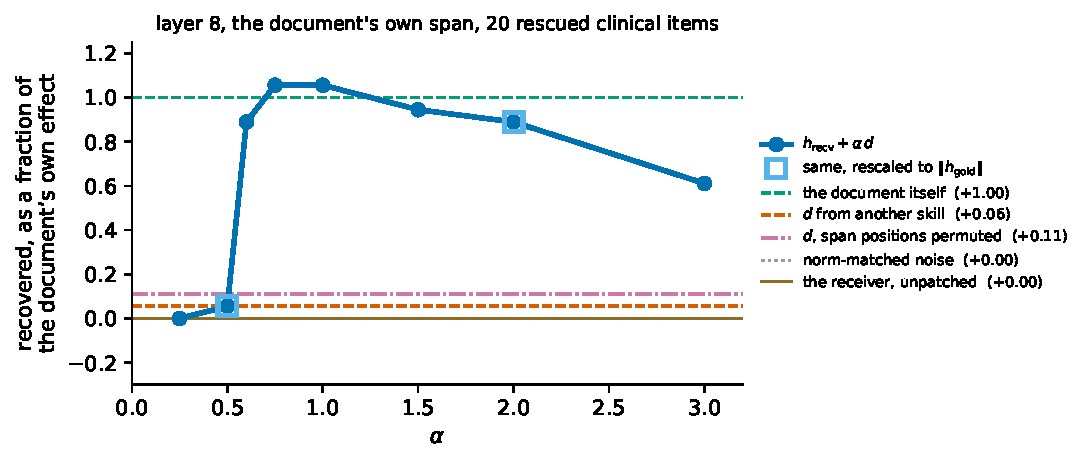
\includegraphics[width=0.9\textwidth]{fig-dose-medcalc.pdf}
\caption{Dose response of the content injection over the document's own span,
layer 8, with its controls. Open squares are the same dose rescaled per position
to the with-document norm; they coincide with the plain arms. Before the
instrument fix; the post-fix dose sweep and norm comparison are in
Appendix~\ref{app:madeof}. The horizontal lines are the three controls and the two
baselines.}
\label{fig:dose}
\end{figure*}

\begin{figure*}[tbp]
\centering
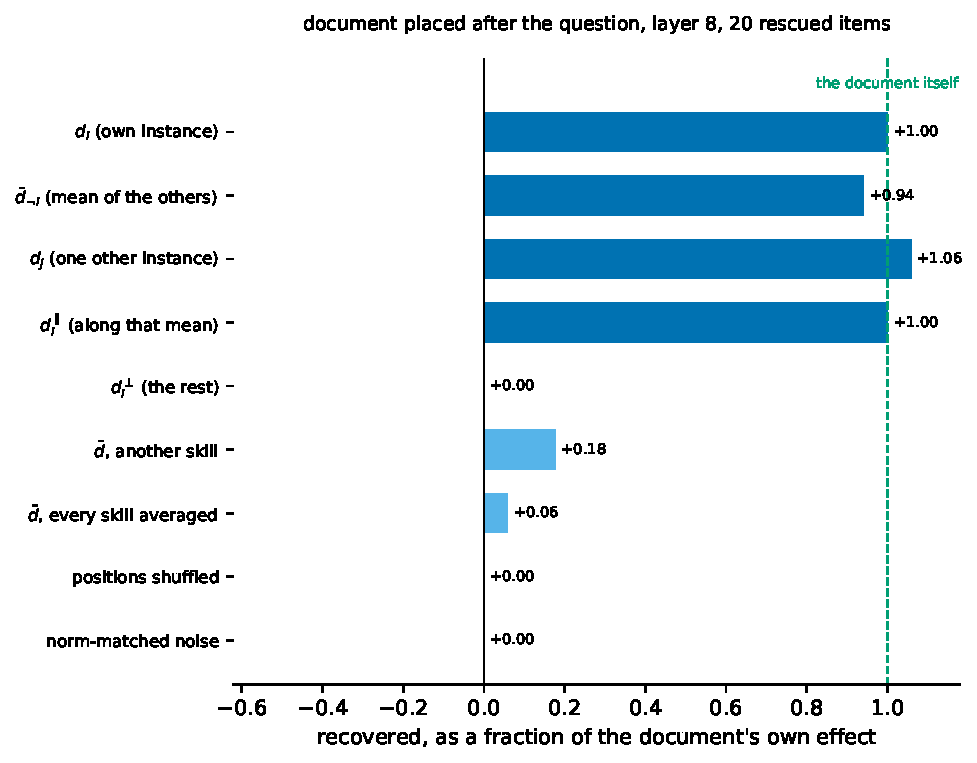
\includegraphics[width=0.72\textwidth]{fig-skilltask-medcalc.pdf}
\caption{What the content vector contains once it is able to contain the task.
Document placed after the question, layer 8, Qwen3-8B, the $40$ rescued items,
plotted as the fraction $\rho$ of Eq.~\ref{eq:rho}, before the instrument fix
(post-fix numbers in Appendix~\ref{app:madeof}). Exact accuracies and
intervals are in Table~\ref{tab:skilltask}, Appendix~\ref{app:tables}.}
\label{fig:skilltask}
\end{figure*}

\begin{figure*}[tbp]
\centering
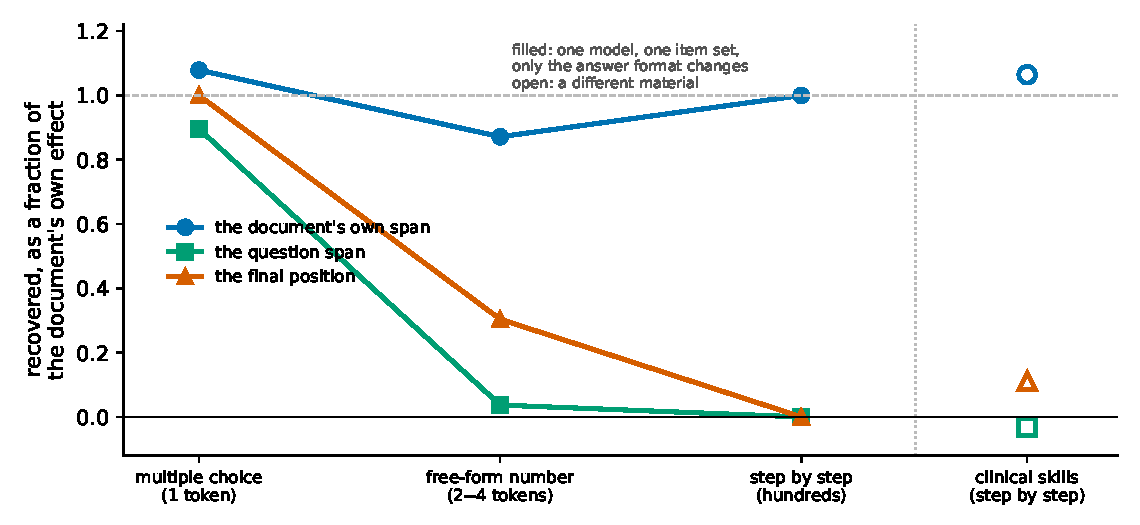
\includegraphics[width=0.92\textwidth]{fig-ladder.pdf}
\caption{What each transplant channel recovers, as a fraction of what the
document itself is worth in that setting, against how many tokens the answer
occupies. Filled markers joined by lines are one model, one item set and one
document with only the answer format changed; the clinical results are open and
deliberately not joined, because that material changes the skill, the task and
the prompt length at once. Plotting fractions rather than raw accuracies is
necessary here: the four settings have donors at $0.550$, $0.467$, $1.000$ and
$0.950$, and comparing raw numbers across them is how an earlier draft came to
report that a \emph{longer} answer made the document-span channel stronger. The
document's own span is flat at $1.00$ across every answer format. The other two
channels collapse as the answer lengthens, and the clinical points land where
the step-by-step column says they should.}
\label{fig:ladder}
\end{figure*}
\subsection{What the carrying vector is made of, in full}
\label{app:madeof}

The vector at the document's span reproduces the document's whole effect, so
what it is composed of is answerable rather than speculative. Four
decompositions, all at layer 8. \textbf{Unless marked ``after the fix'', the
numbers in this subsection come from the ten-calculator development runs made
before the instrument fix}, read against the receiver's $0.175$ and the
document's $0.950$; where a rerun exists it is given and takes precedence.

\paragraph{Not a common shift.} Averaging $\dvec$ over \emph{every} skill in the
set and writing that average gives $\rho = 0.11$, against $1.06$ for the
document's own. What makes this sharp rather than merely negative
is how much of the vector that average is: measured against the same fixed
control, two skills' content vectors have cosine $0.48$--$0.56$ at every depth,
the cosine to the all-skill mean is $0.72$--$0.76$, and $54$--$60\%$ of each
$\dvec$'s energy lies along that mean (Table~\ref{tab:geometry}). \emph{More than
half of the content vector points in a direction that carries nothing.} This is
the span-level counterpart of $\gvec$'s flat $0.098$ at
the final position in \S\ref{sec:decomp}: presence is not what acts, in either
place.

\paragraph{Not a magnitude.} The informative test is the dose curve against its
norm-matched twin. At $\alpha = 2$ the patched state is $2h_{\text{skill}} -
h_{\text{recv}}$, which is $1.76\times$ as long as the with-document state at
layer 8; rescaling it per position back to $\|h_{\text{skill}}\|$ is a $43\%$
change and costs nothing---$\rho = 0.89$ either way. At $\alpha = 0.5$ the state
is $0.88\times$ and rescaling is likewise free ($0.06$ both).

We also ran the reverse, rescaling the with-document states down to the
\emph{receiver's} norm, and it changes nothing ($\rho = 1.06$)---but that arm is
uninformative and we report it only to say so: the two norms differ by $3.5\%$ at
layer 8, so it is barely a manipulation. The $\alpha = 2$ comparison is the one
that carries the claim. The dose curve and its norm-matched twin coincide
at every $\alpha$ we ran ($0.5$: $0.350$ vs $0.350$; $2$: $0.875$ vs $0.875$;
$3$: $0.675$ vs $0.650$). The document's effect is carried by the direction its
span states point in and not by how far along it they go. Norm-matched Gaussian
noise, correspondingly, gives $0.100$, below the receiver.
The norm arms were not rerun after the fix. (The arm listed next to the
transplant in Table~\ref{tab:big40}, $0.73$, is not a norm manipulation: it is
the transfer test's paired control, the document's own $\dvec$ written over only
the prefix another skill's document shares.)

\paragraph{Graded in $\alpha$, and the transition is a step.} After the fix,
on the ten development calculators ($n=16$), $\alpha = 0.4, 0.5, 0.55, 0.6, 0.7,
1, 2$ give $\rho = 0.06, 0.00, 0.06, 0.62, 0.94, 1.00, 0.81$: at the receiver up
to $0.55$ and at the document by $0.7$. Before the fix the same sweep read
$0.17, 0.03, 0.17, 0.88, 0.97, 1.00$ ($n=30$ under a looser restriction), and an
earlier receiver gave $-0.14, +1.03, +1.03, +0.86$ at $\alpha = 0.5, 0.75, 1, 2$
(Figure~\ref{fig:dose}, pre-fix): half the content is no better than none of
it, while three quarters is already most of the effect. Past $\alpha=1$ the
recovery decays slowly rather than breaking, and against the other receiver,
where the fine grid was run, it decays the same way with the norm held fixed
($\alpha=2$: $0.875$ plain against $0.875$ rescaled; $\alpha=3$: $0.675$ against
$0.650$), so what overshooting costs is not the size of the state.

\paragraph{Localised, and in the section one would guess.} Writing $\dvec$ over
only part of the span localises the effect within the document without changing
a single prompt token---the length, the positions and the rotary phases are all
untouched, and only which states are overwritten changes. By halves (pre-fix),
the first gives $\rho = 1.06$ and the second $0.28$, and the first half agrees
with the whole span item by item on $18$ of $20$. By quarters:
\begin{center}
\resizebox{\columnwidth}{!}{%
\begin{tabular}{@{}lccccc@{}}
\toprule
quarter of the span & $n$ & 1st & \textbf{2nd} & 3rd & 4th \\
\midrule
forty calculators, after the fix & $60$ & $0.12$ & $\mathbf{0.56}$ & $0.12$ & $0.12$ \\
ten calculators, after the fix & $16$ & $0.12$ & $\mathbf{0.81}$ & $0.06$ & $0.06$ \\
ten calculators, before the fix & $20$ & $0.28$ & $\mathbf{0.83}$ & $0.11$ & $0.44$ \\
\midrule
controls on the same forty (Table~\ref{tab:big40}) & $60$ & \multicolumn{4}{c}{half dose $0.06$, permuted $0.08$, noise $0.10$} \\
\bottomrule
\end{tabular}}
\end{center}

These documents make that interpretable, because all ten have the same section
order: title, \emph{Required Inputs}, \emph{Computation} (sometimes preceded by a
\emph{Unit Conversion}), \emph{Calculation Tool}, \emph{Example}. Measured in the
units the intervention actually uses---token positions within the span, not
characters---the computational section's \emph{heading} falls at $0.18$--$0.42$
of the span, \emph{Calculation Tool} at $0.47$--$0.70$, and \emph{Example} at
$0.61$--$0.79$. So the second quarter is the \emph{body} of the computational
section, the formula itself, for every one of the ten; the first quarter is the
title, the input list and at most the opening of that section; the third is a
Python function signature and the start of a worked example; the fourth is the
rest of the example.

Read that way the procedural core carries most of the effect, and every other
quarter alone is at the control floor. Two things changed with the fix and the
larger set. The worked example, which read $0.44$ before the fix, reads $0.06$
and $0.12$ after it: \emph{we withdraw the earlier statement that it carries
about half as much as the formula.} And the formula alone, $0.81$ on ten
calculators, is $0.56$ on forty against the whole document's $0.87$, so on the
larger set the other three quarters matter in combination although none matters
alone. The boundaries are approximate and vary by calculator, so we report the
quarters and the section map rather than claiming an exact alignment.

Permuting the span's own positions, which preserves the multiset of vectors and
destroys only the correspondence between them and the tokens, gives $0.08$ on
forty calculators after the fix ($0.21$ before it): nearly all of the effect is
in that correspondence.



\paragraph{Task information, when the vector is allowed to have any.} Under the
prompt format used everywhere else in this paper the question does not arise:
the document precedes the question, so its states are a function of the document
alone and we verified that they agree across a skill's instances (bit for bit at
equal prompt length, cosine $\ge 0.997$ otherwise).
To ask what happens when the vector \emph{can} carry the task, we move the
document behind the question, keeping the answer-format instruction last, and
pad each instance's question with filler tokens so that the document begins at
the same absolute index for every instance of a skill---without which a donor
from another instance would be written at the wrong rotary phase, the error
described in \S\ref{sec:battery}. The format costs almost nothing behaviourally
(the document is worth $0.025 \to 0.925$ instead of $0.025 \to 0.950$) and it
raises the receiver's own baseline to $0.350$.

In that format the vector \emph{can} carry the task, and at layer 8 it does not
use it (read, like everything else here, on the calculators a wrong document
never rescues). After the fix ($n=28$, seven calculators) the instance's own
vector recovers $\rho = 1.00$, the mean of the skill's other instances' vectors
$1.00$, a single other instance's vector $0.96$, and the
orthogonal remainder---everything specific to this patient note---$0.04$. Before
the fix (Figure~\ref{fig:skilltask}) the same arms read $1.00$, $1.00$, $1.06$
and $0.00$. At layer $16$ the picture changes: the instance's own vector still
recovers $0.85$, but the mean of the other instances' vectors $0.63$ and a
single other instance's $0.48$, while the remainder alone stays at $0.04$. By
layer $16$ the doc-last span holds something of the question that other
instances' vectors lack and the remainder cannot supply on its own.

The geometry agrees and says why, before any injection: the cosine between two
instances' $\dvec$ in this format is $0.998$ at layer 0, $0.984$ at layer 8 and
$0.914$ by layer 32, with the fraction of energy along the instance-mean falling
from $0.997$ to $0.880$. At layer 8 the vector is $98\%$ shared, so there is
almost no instance-specific part to use; whether the remaining $12\%$ at layer 32
ever matters is a question we can pose but have not answered.

Everything else replicates across the two prompt orders (pre-fix). Another skill's vector
recovers $0.18$, the mean over every skill $0.06$, the same vectors with the
span's positions permuted $0.00$ and norm-matched noise $0.00$; rescaling to the
receiver's own norm costs nothing ($0.99$); and the first half of the span
carries $1.05$ against the second half's $0.43$, the same concentration in the
formula that the document-first format shows.



\paragraph{Where the document sits changes how deep the handover reaches.}\label{sec:whose:docklast}
Placing the document after the question moves the cliff. We first reported this
as a confirmed rank prediction, on the grounds that the doc-last span's
participation ratio past layer 16 read $28$--$33$ against the doc-first format's
$14$--$17$; \S\ref{sec:depth} shows that both of those numbers are massive
activations rather than representations, and once they are excluded the two
formats have the same, flat dimensionality. The behavioural difference is real
and the rank explanation for it is withdrawn.

The difference is large. On the same items, before the fix, as a fraction of
each format's own range:
\begin{center}
\resizebox{\columnwidth}{!}{%
\begin{tabular}{@{}lccccc@{}}
\toprule
layer & 0 & 4 & 8 & 12 & \textbf{16} \\
\midrule
document first & $1.00$ & $1.07$ & $1.14$ & $1.00$ & $\mathbf{0.14}$ \\
document last  & $0.99$ & $1.11$ & $1.00$ & $0.93$ & $\mathbf{0.80}$ \\
\bottomrule
\end{tabular}}
\end{center}

Both formats carry the document's whole effect through layer 12. At layer 16 the
document-first format carries a seventh of it and the document-last format four
fifths; the latter's own cliff comes later, between layers 16 and 20 ($0.82$ to
$0.35$). Under causal masking a document placed first cannot see the question
and a document placed last can, so the doc-last span's states are already
question-conditioned when they are captured---which is the obvious candidate
explanation, and is not one we have tested.

After the fix the layer-$16$ contrast holds: $0.85$ with the document last
($n=28$) against $0.19$ with it first on forty calculators. Before the fix, at
layers $0, 12, 16, 20$ in the document-last format the mean of the skill's other
instances tracked the instance's own ($1.06/1.00$, $0.88/0.94$, $0.82/0.82$,
$0.29/0.35$) with the remainder at the receiver; the rerun at layer $16$
($0.63$ against $0.85$, above) does not reproduce that agreement, so we no longer
claim that the instance-specific part never matters at depth---only that it does
nothing alone.

What this rules out is the reading in which the handover depth is a fixed
property of the network: it moves under a change to the prompt that leaves the
model, the document and the items alone.

\subsection{Depth, sufficiency and necessity, in full}
\label{app:depth}

\begin{table*}[tbp]
\caption{Centred participation ratio of the content matrix across the
document's span on Qwen3-8B, measured four ways, medians over $96$ items from
all $48$ documents (the plain column is bimodal, so its mean describes no
item). The first column is the quantity usually reported and the only one that
collapses. The last two columns say why---they are properties of the state
itself, not of the difference: at layer $16$ one token in $35$ of $48$
documents acquires a state $153$ times (median) the span's norm, carried by two
fixed hidden dimensions, and the top eight dimensions then hold $98\%$ of the
variance. Removing four positions out of four hundred, or normalising each
position to unit length, removes the collapse entirely.}
\label{tab:prdiag}
\centering
\small
\setlength{\tabcolsep}{4pt}
\begin{tabular}{@{}rrrrrrr@{}}
\toprule
& \multicolumn{4}{c}{participation ratio, computed\ldots} & \multicolumn{2}{c}{massive activations} \\
\cmidrule(lr){2-5}\cmidrule(l){6-7}
layer & as usual & drop 4 loud & unit-norm. & drop 8 dims & $\max/\mathrm{med}\,\|h\|$ & top-8 var. \\
\midrule
$8$ & $97.7$ & $97.0$ & $103.4$ & $114.2$ & $1.5$ & $4.9\%$ \\
$12$ & $68.1$ & $70.0$ & $79.4$ & $88.9$ & $1.6$ & $5.6\%$ \\
$14$ & $76.3$ & $76.8$ & $83.7$ & $93.7$ & $1.6$ & $5.3\%$ \\
$16$ & $1.0$ & $85.2$ & $91.4$ & $36.6$ & $152.7$ & $97.7\%$ \\
$20$ & $1.1$ & $84.9$ & $89.1$ & $70.1$ & $94.2$ & $94.8\%$ \\
$28$ & $2.5$ & $62.4$ & $70.9$ & $100.8$ & $27.2$ & $64.7\%$ \\
$34$ & $32.4$ & $34.2$ & $43.0$ & $113.4$ & $1.3$ & $15.7\%$ \\
\bottomrule
\end{tabular}

\end{table*}


On the clinical material the two questions---\emph{can} the document's states be
handed over at layer $L$, and \emph{is} the model still reading them at layer
$L$---give different answers, and the disagreement is the informative part.

Sufficiency, on forty calculators after the instrument fix ($n=60$, twenty
calculators after the restriction): a single layer's worth of the span reproduces
$\rho = 1.04, 0.94, 0.85, 0.77$ at layers $0, 4, 8, 12$ and then
$0.28, 0.19, 0.19, 0.15$ at $14, 15, 16, 20$. The first, pre-fix sweep on twenty
items (Table~\ref{tab:realspandepth}) has the same shape: $1.00$ at $0$ and $12$,
three quarters at $13$--$14$, $0.14$ at $15$ and $16$, nothing by $24$.

Necessity, from cumulative attention knockout with the full chain of thought
decoded ($n=40$ rescued items, twenty calculators): masking every position's
attention to the document's tokens from layer $L$ to the end leaves
$0.08$--$0.15$ of the items correct for every $L \le 20$ except $L=4$ ($0.33$),
then $0.38$ at $24$, $0.75$ at $28$ and $0.95$ at $32$. An earlier knockout run
capped generation at 400 tokens, truncating the chain of thought so that even the
unmasked prompt scored $0.50$; it is superseded and not used. The model is still
reading the document long after a single-layer handover has stopped working.

\paragraph{It is not that one layer is too few: the channel closes.} The
natural reading of the cliff is that a single layer stops being enough, since
writing the span at \emph{every} layer at once still recovers $0.950$. It is
wrong, and one experiment separates the two. We write the span at every layer in
a window $[\ell_{\text{lo}}, \ell_{\text{hi}}]$ and nowhere else.
The complete corrected window run uses a different receiver from the span
battery. Using its own baselines and group screen retains $222$ items from
$21$ calculators. Recovery is $0.95$ for $8$--$11$, $0.81$ for $12$--$15$,
$0.22$ for $14$--$19$ and $0.10$ for $16$--$35$, with an exact identity
control at $0.00$. The final window matches layer $16$ alone. Earlier versions
incorrectly merged this run with the span battery's receiver baselines,
producing $n=137$ and incompatible normalisation; those estimates are
superseded. Repeating the injection across late layers does not restore the
early-window recovery, although the window and single-layer sweeps are not
directly paired across receivers.

This is worth stating as a negative constraint on any mechanism, including the
one we tried to give it. Whatever ends at layer $15$ is not a capacity that more
depth can compensate for.

\paragraph{The span's representation does \emph{not} become a summary, and the
measurement that says it does is an artefact.} The obvious explanation for the
cliff is that the span has by then been compressed, and the obvious measurement
agrees: the centred participation ratio of the span's states, which counts the
directions its positions differ in, reads $64$ at layer $12$ and $17$ at layer
$16$---the same interval. We report it here because we believed it, built a
mechanism on it, and it is wrong.

Three things give it away. It is a step and not a slope: the span states'
participation ratio lies between $47$ and $75$ for every item at layer $14$ and
below $5$ for thirty-four of forty at layer $16$ (Table~\ref{tab:prdiag}), and
the content matrix's mean of $17$ at layer $16$ describes no item---thirty-two
of forty read below $5$ and the other eight at $81$. A participation ratio of
$1.0$ over four hundred positions asserts that the centred span is rank one,
which is not a statement one can make about four hundred tokens of text that
the model still has to continue. And the collapse is absent in Qwen3-0.6B and
Qwen3-1.7B at every depth ($45$--$99$, no item below $5$) although their
transplant cliff is in the same place in relative depth
(\S\ref{sec:ladder}).

The cause is measurable and known. At layer $16$---and at no earlier layer---one
token in $34$ of $40$ documents acquires a state whose norm is $99$ to $180$ times the
span's median, carried by hidden dimensions $2276$ and $676$, the same two in
all $34$. That is the massive-activation phenomenon of
\citet{sun2024massive}, which appears at a single layer per model family
\citep{shi2026melayer}; in this model the loud token is a late delimiter inside
the document rather than the sequence start. A centred spectrum is then owned by
that one position: the top eight dimensions hold $97.7\%$ of the variance at
layer $16$ against $5.4\%$ at layer $14$. Removing the four loudest positions
out of four hundred restores the participation ratio to $66$; unit-normalising
each position restores it to $68$; removing the top eight dimensions gives $27$.
Measured any of those three ways, the span's dimensionality is
\emph{flat} from layer $0$ to layer $28$ and only falls in the last few layers
(Table~\ref{tab:prdiag}).

So the honest statement is the narrower one. The single-layer handover dies
between layers $14$ and $16$; the document's representation does not lose
dimensionality there; we do not know what it does lose. What \S\ref{sec:rank}
establishes is a different and still causal fact---how many directions the
injected object needs---and in the small pre-fix repeats at layers $12$ and
$16$ that number is not lower either (Appendix~\ref{app:rank2}).



\paragraph{A warning about participation ratio on residual streams.} Effective
rank, participation ratio and intrinsic dimension are routinely computed on
residual-stream activations, including in work that reports collapses with depth
\citep{fernando2026residualspectral, sarkar2026causaldim}. Massive activations
begin at a fixed layer, are carried by a handful of dimensions at a handful of
positions, and are large enough to own a spectrum by themselves. Any such
measurement that does not exclude them will report a collapse at exactly the
emergence layer whether or not the representation has changed. Our own draft did.
We recommend reporting the per-position norm ratio alongside any spectral
statistic; here its median goes from $1.6$ to $150$ across the layer in question.
\subsection{Where in the network the content is readable, in full}
\label{app:where}

Transplanting one group of positions from the with-document forward into the
without-document forward asks where the content can be \emph{read from}; masking
attention to the document asks where it is still being \emph{read}. In the
multiple-choice format the first question gives three windows that hand off
cleanly (Figure~\ref{fig:windows}, Appendix~\ref{app:decomp}): the document's own
688 tokens work at layers 0--10 and fall off a cliff at 11, the question's 42--47
tokens work at 11--16, and the final prompt position works at 21--27. The handoff
is not an artefact of a shared analysis---the two experiments were run
independently---and at layer 11 the document-span channel drops from $0.308$ to
$0.128$ while the question-span channel rises from $0.231$ to $0.308$. The
windows survive a change of model and not a change of format
(Table~\ref{tab:windows2}): in free-form, on the same model and items, the
question span recovers $0.000$--$0.025$ at every one of 12 layers.

The second question gives a different shape. No single pathway is necessary:
masking only the final position's attention to the document costs nothing
($0.436$ against $0.436$) and masking only the question span's leaves $0.282$,
so the read is redundantly distributed, as \citet{jit2025taskrepr} report for
task representations generally. What is necessary is the document's own tokens.
On third-party skills, making them unattendable for the whole forward takes
accuracy from $0.550$ $[0.400, 0.700]$ to $0.075$ $[0.000, 0.175]$, against
$0.025$ $[0.000, 0.075]$ with no document in the prompt at all---ninety per cent
of the benefit, with the remainder inside the no-document interval. Masking an
equal-length span of the patient note instead costs less, $0.150$
$[0.050, 0.275]$. A genuinely inert length-matched control cannot be built here,
since the only other long span is the data the task needs, so this bounds
``removing 900 tokens'' loosely but in the right direction.

Single-layer knockouts measure nothing on a 688-token span, because a layer
denied the read recovers it one layer later; cumulative knockouts are required
and are what we report. Cumulatively, the document stops being needed at layer
22 of 28 when the answer is one token, and is still being read at $83\%$ depth
when the answer is several hundred---the necessity-side view of
\S\ref{sec:onepos}.



\subsection{What the content component belongs to, in full}
\label{app:whose}
\label{app:belongs}

If $\dvec$ were a ``skill vector'' it would be reusable: extracted from one task
it would work on another. Its \emph{direction} is reusable. Its \emph{effect}
is not, and the gap between those two statements is the finding.

\paragraph{The vector that carries contains no task information, and we check
rather than argue it.} Everything in this section so far is about the vector at
the final position, the one that does not act. The vector that does act---the
content component over the document's own span---has a property that makes the
question sharp. In the prompt format the behavioural runs use, the document
precedes the question, so causal masking makes the document's hidden states a
function of the system text and the document alone. Within one skill the
document is byte-identical across its instances, so $\dvec(\text{span})$ should
be \emph{the same tensor} for every instance of that skill.

It is. Across the ten calculators in the causal set, the document span occupies
token positions $43$ to $43+m$ in every prompt, the token ids there are
pairwise identical across instances (zero differing positions in $40$ notes),
and truncating two prompts to the end of the span and re-running the forward
gives a relative difference of $0.0$. In the full prompts the states differ by a
relative $3.5\times10^{-3}$ at layer 0 and $8.6\times10^{-3}$ at layer 8, with
zero positions below cosine $0.999$---accumulated bf16 rounding from the
differing sequence lengths, not content. The decode arms show the same thing
behaviourally: the mean of the \emph{other} instances' vectors and the
instance's own agree to three decimals at every running mean, and the component
of $\dvec_i$ orthogonal to that mean lands exactly on the receiver's baseline.

So the vector that reproduces the document's entire effect is a function of the
document and of nothing else. Whatever a ``skill vector'' should be, this one is
not a joint encoding of skill and task; it is the skill, and it is sufficient.
The complementary experiment---moving the document behind the question so that
its states \emph{can} see the task---is \S\ref{sec:whose:docklast}.

\paragraph{The direction differs by skill; the effect does not transfer.}
On the clinical material each skill has 20 instances, so ``same skill, different
task'' is directly measurable. Content vectors from different patient notes under
the same calculator have cosine $0.789$ at layer 20 and $0.876$ at layer 30;
vectors from different calculators, $0.320$ and $0.653$ ($n=40$, Qwen3-8B). On
the synthetic tier the analogous split is by conversion family, $0.869$ within
against $0.705$ across at the last layer. The direction of $\dvec$ carries the
identity of the document, increasingly so with depth. Its effect at the final
position does not: injecting the mean direction $\bar{\dvec}$, or another item's
$\dvec_j$, repairs $0.000$ at every one of 16 layers in the free-form format
against $0.268$ for the item's own, and in multiple choice reaches $0.098$,
$0.293$ and $0.049$ for the mean, a same-family and a different-family donor
against $0.780$ for $\dvec_i$ (Table~\ref{tab:causal}). The one band where a
donor looks transferable is the band \S\ref{sec:traps} identifies independently
as one where the forward pass is damaged and every condition rises together.

\paragraph{Nothing about it distinguishes rescued items from persistent
failures.} The norms and angles of $\dvec$ and $\gvec$ agree to three digits
across the two cells (layer 30, 8B, real skills: $\|\dvec\|$ $189.4$ vs $185.4$,
$\cos(\dvec,\gvec)$ $-0.469$ vs $-0.468$). A representational-similarity measure
over the question span does separate them under the gold skill at layers 10--16
($-0.0037$ to $-0.0070$, non-overlapping intervals, $n=150+150$)---and separates
them just as much under a length-matched \emph{wrong} skill ($-0.0035$ to
$-0.0056$). Zero layers pass a control the design required in advance, so what
looked like a signature of ``the skill worked here'' is a signature of ``a
document is present'': \S\ref{app:geometry}'s trap one register down, and the
reason we report a causal channel rather than a similarity score.

\paragraph{The content component's size depends on where it is written.} At the
final position the content component is a $6\%$ perturbation of the state it
displaces at layer 6 ($\|\dvec\|=2.3$ against $\|h_{\text{no}}\|=37.3$), rising
to $51\%$ by layer 35---and it is causally inert at every one of them. Over the
document's own span the same difference of the same two conditions is $95\%$ to
$115\%$ of the state at every depth (Table~\ref{tab:geometry})---a replacement
rather than a nudge---and it is causally complete (\S\ref{sec:battery}). What
distinguishes the two places is not how much the document is written into them;
it is whether what is written is the whole of what the downstream computation
reads.

\paragraph{The shared part carries the norm, not the effect.} Between $73\%$ and $99.7\%$ of each item's
$\dvec_i$ lies along the shared mean direction, depending on layer
(Table~\ref{tab:geometry-tierA}); the remainder occupies an effective 3--18 dimensions
out of 2048--4096. The reusable part is almost all of the norm and, in free-form
answering, none of the effect; in multiple choice it is worth $0.06$ of the
$0.79$ the item's own vector achieves. A single vector per skill is therefore a
fair description of
what the injection \emph{looks like} and a wrong description of what it
\emph{does}, which is the same inversion as \S\ref{app:geometry} one level
down.



